\documentclass{beamer}

\usepackage{amsfonts}
\usepackage{amsmath}
\usepackage{longtable}
\usepackage{csquotes}
\usepackage{standalone}

\usepackage{graphicx}
\graphicspath{{../pictures/}}

\usepackage{tikz}
\usetikzlibrary{shapes, calc, arrows, decorations.markings,
  decorations.pathmorphing, decorations, patterns, chains, snakes,
  backgrounds, positioning, fit, petri}
\newcommand{\inputpicture}[1]{\input{../drawings/#1}}

\usepackage{listings}
\lstset{language=C, basicstyle=\ttfamily, breaklines=true, keepspaces=true,
  keywordstyle=\color{blue}}

\usepackage{bytefield}

\usefonttheme{professionalfonts}
\usefonttheme{serif}
\usepackage{fontspec}
\setromanfont{CMU Serif}
\setsansfont{CMU Sans Serif}
\setmonofont{CMU Typewriter Text}

\usepackage{hyperref}
\hypersetup{colorlinks=true, linkcolor=black, filecolor=black, citecolor=black,
  urlcolor=blue , pdfauthor=Evgenii Iuliugin <yulyugin@gmail.com>,
  pdftitle=Fundamentals of Full-Platform Simulation}

\usepackage{underscore}
\usepackage{amsthm}

\subtitle{Fundamentals of Full-Platform Simulation}
\subject{Lecture}
\date{\today}

\author[Evgenii Iuliugin]{
  Evgenii Iuliugin, \small{\href{mailto:yulyugin@gmail.com}{yulyugin@gmail.com}}}
\typeout{Copyright 2021 Evgenii Iuliugin}

\usetheme{Madrid}
\setbeamertemplate{navigation symbols}{}

\makeatletter
\setbeamertemplate{footline}{%
  \leavevmode%
  \hbox{%
    \begin{beamercolorbox}[wd=.15\paperwidth,ht=2.25ex,dp=1ex,center]{author in head/foot}%
      \usebeamerfont{author in head/foot}\insertshortauthor\expandafter\ifblank\expandafter{\beamer@shortinstitute}{}{~~(\insertshortinstitute)}
    \end{beamercolorbox}%
    \begin{beamercolorbox}[wd=.77\paperwidth,ht=2.25ex,dp=1ex,center]{title in head/foot}%
      \usebeamerfont{title in head/foot}\insertshorttitle
    \end{beamercolorbox}%
  }%
  \begin{beamercolorbox}[wd=.08\paperwidth,ht=2.25ex,dp=1ex,right]{date in head/foot}%
    \usebeamerfont{date in head/foot}%
    \usebeamertemplate{page number in head/foot}%
    \hspace*{2ex}
  \end{beamercolorbox}
  \vskip0pt%
}
\makeatother

\newcommand{\startslides}{
  {\setbeamertemplate{footline}{}
  \begin{frame}
      \maketitle
  \end{frame}
  }

  \addtocounter{framenumber}{-1}

  \begin{frame}{\inserttitle}
      \tableofcontents
  \end{frame}
}

\newcommand{\finalslide}{{
  \setbeamertemplate{footline}{}

  \begin{frame}

  {\huge{Thank you!}\par}

  \vfill
  Slides and material are available at
  \url{https://github.com/yulyugin/sim-lectures}
  \vfill

  \tiny{\textit{Note}: All trademarks are the property of their respective
    owners. The presented point of view reflects the personal opinion of
    the author.

    %All the materials are licensed under the Creative Commons
    %Attribution-NonCommercial-ShareAlike 4.0 Worldwide. To view a copy of this
    %license, visit \url{http://creativecommons.org/licenses/by-nc-sa/4.0/}.
  }
  \end{frame}
}\addtocounter{framenumber}{-1}}


\usepackage{tikz}
\usetikzlibrary{shapes, calc, arrows, decorations.markings, decorations.pathreplacing, decorations.pathmorphing, decorations, patterns, chains, snakes, backgrounds, positioning, fit, shadows}
\title{Processor instruction simulation}

\begin{document}

\section{Start}
\startslides

\begin{frame}{Simulated System}
\centering
\vfill
\inputpicture{cpu-mem}
\vfill
\end{frame}

\section{Interpretation Pipeline}

% TODO: This is not a pipeline! Add a proper pipeline picture.
% s/pipeline/execution stages/g

\begin{frame}{Basic 5-Stage Pipeline}
\centering
\inputpicture{interpreter-cycle}
\end{frame}

\begin{frame}[fragile]{Switched interpreter}
\begin{lstlisting}
while (run) {
    raw_code = fetch(PC);
    (opcode, operands) = decode(raw_code);
    switch (opcode) {

    case opcode1:
        func1(operands); PC++; break;

    case opcode2:
        func2(operands); PC++; break;

    /*...*/
    }
}
\end{lstlisting}
\end{frame}

\subsection{Fetch}

\begin{frame}[fragile]{Fetch}
\texttt{data = mem[pc];}\pause
\vfill
Do not forget about address translation:
\begin{lstlisting}
paddr = v2p(pc); // pc is a virtual address
data = mem[paddr];
\end{lstlisting}
\end{frame}

% TODO: Add a slide about paging. People don't know about it at the moment.

\begin{frame}{Fetch}
<<Simple>> memory read?
\pause\bigskip
\begin{itemize}
\item Non-execute page.
\pause\bigskip
\item Unaligned accesses cause effects on some architectures.
\pause\bigskip
\item Cross-page accesses. \\
The pages may have different access rights.
\end{itemize}
\end{frame}

\subsection{Decode}

\begin{frame}{Decode}
Decoding --- translation of instruction data from machine code to internal
(high-level) representation suitable for further analysis.
\end{frame}

\begin{frame}{Example 1: RISC-V}
\centering
\includegraphics[width=.9\textwidth]{risc-v-formats}

\tiny{Source: The RISC-V Instruction Set Manual, Volume I: Unprivileged ISA,
      Document Version 20191213, page 16}
\end{frame}

\begin{frame}[fragile]{Example 1: RISC-V decoder (1/3)}
\begin{lstlisting}
#define BIT_FIELD(v, e, s) \
    (v >> s) & ((1 << (e - s + 1)) - 1)

static inline int32_t
sign_extend(uint32_t v, int width) {/* ... */};

typedef struct decode {
    uint32_t opcode;
    uint32_t rd;
    uint32_t rs1;
    uint32_t rs2;
    int32_t  imm;
    uint32_t funct3;
    uint32_t funct7;
} decode_t;
\end{lstlisting}
\end{frame}

\begin{frame}[fragile]{Example 1: RISC-V decoder (2/3)}
\begin{lstlisting}
decode_t
decode(uint32_t raw) {
    uint32_t op = BIT_FIELD(raw, 6, 0);
    switch (type(op)) {
    case I_type:
         return decode_i_type(raw);
    case R_type:
         return decode_r_type(raw);
    /../
    }
}
\end{lstlisting}
\end{frame}

\begin{frame}[fragile]{Example 1: RISC-V decoder (3/3)}
\begin{lstlisting}
decode_t
decode_i_type(uint32_t raw) {
    uint32_t op = BIT_FIELD(raw, 6, 0);
    uint32_t rd = BIT_FIELD(raw, 11, 7);
    uint32_t funct3 = BIT_FIELD(raw, 14, 12);
    uint32_t rs1 = BIT_FIELD(raw, 19, 15);
    int32_t imm = sign_extend(
        BIT_FIELD(raw, 31, 20), 12);

    return (decode_t){.op = op, .rd = rd,
                      .funct3 = funct3, .rs1 = rs1,
                      .imm = imm};
}
\end{lstlisting}
\end{frame}

\begin{frame}{Example 3: Intel\reg~IA-32}
\centering
\includegraphics[width=.9\textwidth]{ia32-evex}

\tiny{J.C.S. Adrian et al. Systems, Apparatuses, and Methods for Blending Two
      Source Operands into a Single Destination Using a Writemask. US Patent
      Application Publication. \No~2012/0254588 A1}
\end{frame}

\begin{frame}{What to Fetch From Machine Code?}
\begin{centering}
\inputpicture{instruction-anatomy}
\end{centering}
\vfill
Input: machine code.

Output:
\begin{itemize}
\item Success, failure, not enough data.
\item In case of success: instruction length.
\item In case of success: information about operands.
\item In case of success: simulation routine.
\end{itemize}
\end{frame}

\begin{frame}{Decode}
\begin{itemize}
\item Decoders are usually generated from ISA description.
\item In general: classical problem of parser/synax analyser construction.
\item In practice: special tools and languages.
\item Example: Intel\reg~XED (x86 encoder-decoder). \url{https://github.com/intelxed/xed}
\end{itemize}
\end{frame}

\begin{frame}{Decode: harsh reality}
\begin{itemize}
\item Variable instruction length. Intel\reg~IA-32: from 1 to 15 bytes. How many bytes to decode at once?
\item Decoding results depends of prefixes and execution mode. Example: 0x40-0x4f in Intel\reg~IA-32/Intel\reg~64/AMD64.
\end{itemize}
\end{frame}

\begin{frame}{Disassemble}
\begin{itemize}
\item Disassemble --- translate from machine code into human readable
  representation (mnemonic, assembly).
\item Encode (assemble) --- translate from mnemonic to machine code.
\end{itemize}
\end{frame}

\subsection{Execute}

\begin{frame}{Execute}
\begin{itemize}
\item Basic block --- simulation function for one instruction (a.k.a.~service routine).
\item Service routines are tipically written in high-level programming
  languages: portable solution.
\item Generators are often used.
\item Example: SimGen --- single discription is used to generate decoder,
  disassembler and service routines.
\end{itemize}
\end{frame}

\begin{frame}[fragile]{Simulated state}
\begin{lstlisting}
typedef struct {
    uint32_t pc;

    uint32_t regs[16];

    bool z_flag;
    bool n_flag;
    bool o_flag;
    bool c_flag;
} cpu_t;
\end{lstlisting}
\end{frame}

\begin{frame}[fragile]{Example: ADD reg reg reg}
\begin{lstlisting}

void add32_rrr(cpu_t *cpu, int src1, int src2, int dst) {
    cpu->regs[dst] = cpu->regs[src1]
                   + cpu->regs[src2];
\end{lstlisting}
\pause

\begin{lstlisting}
    cpu->z_flag = cpu->regs[dst] == 0;
    cpu->n_flag = cpu->regs[dst] & (1 << 31);
    cpu->o_flag = cpu->regs[dst] < 
            MAX(cpu->regs[src1], cpu->regs[src2]);
    cpu->c_flag = calc_c_flag(cpu->regs[src1],
                              cpu->regs[src2]);
}
\end{lstlisting}
\end{frame}

\begin{frame}{Intel\reg~IA-32 CALL}
\centering
\includegraphics[width=\textwidth]{ia32-call}

\tiny{Source: Intel\reg~64 and IA-32 Architectures Software Developer’s Manual,
      Order Number: 325462-073US, pages 716-732.}
\end{frame}

\subsection{Memory}

\begin{frame}[fragile]{Memory}
<<Ordinary>> memory access:
\vfill
\begin{lstlisting}
write_mem(cpu, dst_addr, data, size);
data = read_mem(cpu, dst_addr, size);
\end{lstlisting}
\pause\vfill
\begin{itemize}
\item Attempt to change read-only memory,
\item Unaligned address,
\item Cross-page access.
\end{itemize}
\end{frame}

\subsection{Exceptions}

\begin{frame}{Accurate Pipeline}
\centering
\resizebox{9cm}{7cm}{\inputpicture{interpreter-cycle-exception}}
\end{frame}

\begin{frame}{Classification}
\begin{itemize}
\item Exception --- synchronous, without repeating of current instruction.
\item Fault --- synchronous, with repeating of current instruction.
\item Trap --- synchronous, without repeating of current instruction, intentoinal.
\item Interrupt --- external, asynchronous.
\item Abort --- external, asynchronous, no return point.
\end{itemize}
\end{frame}

\subsection{Write-Back}

\begin{frame}{Write-Back}
\begin{itemize}
  \item Processor state should be updated after all excecption checks to avoid
    partially changed state.
  \bigskip
  \item Advance \texttt{\$PC}:
  \pause\bigskip
  \begin{itemize}
    \item For most instructions: \texttt{\$PC += instruction_length}. \\
    Exception: \texttt{REP MOVS}.
    \pause\bigskip
    \item Explicit \texttt{\$PC} update --- control-flow instructions:
    \begin{itemize}
      \item (Un)conditional (In)direct Jump/Branch,
      \item Call/Return (subroutine).
      \item System call/return.
      \item ...
    \end{itemize}
  \end{itemize}
\end{itemize}
\end{frame}

\section{Improved Interpretation}

\begin{frame}{Interpretation Pros and Cons}
\begin{itemize}
\item Implemented in high-level language --- portable.
\item Simple structure: reliable, extensible, re-usasble.
\item (Extremely) low simulation speed.
\end{itemize}
\end{frame}

\begin{frame}[fragile]{Where Is the Time Spent?}
\begin{lstlisting}
start: interruption = false;
while (!interruption) {
    raw_code = fetch(PC);
    (opcode, operands) = decode(raw_code); // <-- here
    switch (opcode) { // <-- and here
    case opcode1:
        func1(operands); PC++; break;
    case opcode2:
        func2(operands); PC++; break;
    /*...*/
    }
}
handle_interruption();
goto start;
\end{lstlisting}
\end{frame}

\begin{frame}[fragile]{Threaded Interpretation}
Jump right to the next instruction instead of start of the loop:
\bigskip
\begin{lstlisting}
func0: /* simulate instr0 */; PC++;
  next_opcode = decode(fetch(PC));
  goto func_ptr[next_opcode];
func1: /* simulate instr1 */; PC++;
  next_opcode = decode(fetch(PC));
  goto func_ptr[next_opcode];
func2: /* simulate instr2 */; PC++;
  next_opcode = decode(fetch(PC));
  goto func_ptr[next_opcode];
\end{lstlisting}

\tiny\url{http://stackoverflow.com/questions/11227809/why-is-processing-a-sorted-array-faster-than-an-unsorted-array}
\end{frame}

\begin{frame}{Cached Interpretation}
\begin{itemize}
\item Usually guest code is static.
\item It's highly probable that an instruction with some \texttt{\$PC} will be
  executed many times.
\item Why decode every time?
\item Solution: create a cache mapping instruction address to decode data.
\end{itemize}
\end{frame}

\begin{frame}[fragile]{Cached Interpretation}
\begin{lstlisting}
while (!interruption) {
  if (operation = cache[PC]); // shortcut
  else { // not cached, full path
    operation = decode(fetch(PC));
    cache[PC] = operation; // cache the result
  }
  switch (operation) {
     /* ... */
  }
}
\end{lstlisting}
\end{frame}

% TODO: slide with diagram.

\begin{frame}{Cached Interpretation}
\begin{itemize}
\item Cache size is limited.
\item Old data needs to be removed from the cache.
\item Code modifications need to be tracked. Otherwise cache will have invalid
  data.
\end{itemize}
\end{frame}

\begin{frame}{What Was Optimized in Interpreter}
\begin{itemize}
\item \textbf<1>{Fetch} {$\leftarrow$ optimized}
\item \textbf<1>{Decode} {$\leftarrow$ optimized}
\item \textbf<2>{Execute} {$\rightarrow$ to be optimized}
\item \textbf<2>{Memory} {$\rightarrow$ to be optimized}
\item \textbf<2>{Write-Back} {$\rightarrow$ to be optimized}
\end{itemize}
\end{frame}

\section{Binary translation}

\begin{frame}{Translation, Compilation, Decompilation}
\begin{itemize}
\item \textbf{Translation} --- \textit{generic term} describing a process of
  code conversion from one programming language into another.
\item \textbf{Compilation} --- \textit{translation} from high-level programming
  language into low-level programming language.
\item \textbf{Decompilation} --- \textit{translation} from low-level programming
  language into a high-level programming language.
\end{itemize}
\end{frame}

\begin{frame}{Binary Translation}
\begin{itemize}
\item Input: guest machine code.
\item Output: host machine code.
\item \textbf{Binary translation, BT} --- translation of guest software written in
  guest ISA into equivalent code in host ISA.
\item What for? \pause Repetitive execution of translation result. Optimizations.
\end{itemize}
\end{frame}

\begin{frame}{Static and Dynamic Binary Translation}
\begin{itemize}
\item \textit{Static} binary translator converts a target executable file
  without running it.
\item Result of static BT is saved on disk.
\item It is very difficult to do correctly.
\vfill
\item \textit{Dynamic} binary translation happens during simulation.
\item Result of dynamic BT is saved in memory.
\item Dynamic BT can adopt to program's run-time environment.
\item Dynamic BT alternates with execution of the generated code.
\end{itemize}
\end{frame}

\begin{frame}{Stages of Dynamic Binary Translation}
\centering
\inputpicture{dynamic-bt}
\end{frame}

\subsection{Template-Based Translation}

\begin{frame}{Algorithm 1: Template-Based Translation}
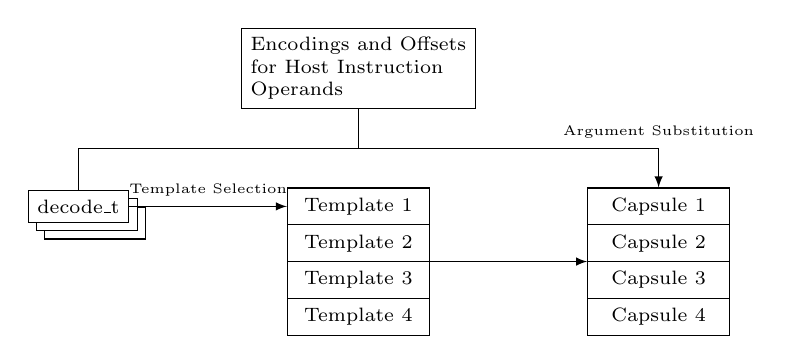
\begin{tikzpicture}[font=\scriptsize, >=latex, node distance=2.cm]

\node[draw, double copy shadow={shadow xshift=3pt,shadow yshift=-3pt}, fill=white] (decode) {decode_t};
\node[rectangle split, rectangle split parts=4, draw, right=of decode, anchor=text west, minimum width=1.8cm] (templates-raw) {Template 1\nodepart{two} Template 2\nodepart{three} Template 3\nodepart{four} Template 4};

\node[rectangle split, rectangle split parts=4, draw, right=of templates-raw, minimum width=1.8cm] (templates) {Capsule 1\nodepart{two} Capsule 2\nodepart{three} Capsule 3\nodepart{four} Capsule 4};

\node[draw, above=1cm of templates-raw, align=left] (md) {Encodings and Offsets\\for Host Instruction\\Operands};

\draw[->] (decode) -- (templates-raw.text west) node[midway, above]{\tiny Template Selection};
\draw[->] (templates-raw) -- (templates);
\coordinate[above=0.5cm of templates] (junction);
\draw[->] (decode) |- (junction) -- (templates) node[pos=0, above]{\tiny Argument Substitution};
\draw[] (md) |- (junction);
\end{tikzpicture}
\end{frame}

\begin{frame}[fragile]{Algorithm 1: Template-Based Translation}
\begin{tiny}
\begin{itemize}
    \item start_addr --- guest code's start address,
    \item start_buf --- host buffer.
\end{itemize}
\end{tiny}

\begin{lstlisting}
translate(start_addr, start_buf) {
    PC = start_addr; bufptr = start_buf;
    while (!enough) {
        instr = fetch(PC);
        (opcode, operands) = decode(instr);
        (template, length) = templates[opcode];
        memcpy(bufptr, template, length);
        patch_operands(bufptr, operands);
        PC += instr_length;
        bufptr += length;
    }
    memcpy(bufptr, glue_capsule, glue_length);
}
\end{lstlisting}
\end{frame}

\begin{frame}[fragile]{Algorithm 1: Execution}

\begin{lstlisting}
execute(start_buf) {
    load_simulated_state();
    goto start_buf;
}
\end{lstlisting}
\pause
or
\begin{lstlisting}
typedef void (*fblock)(void);
execute(start_buf) {
    load_simulated_state();
    ((fblock)start_buf)();
}
\end{lstlisting}
\end{frame}

% TODO: Add JIT-template for the same ADDQ instruction

\begin{frame}{Capsule}
\begin{small}
\begin{tabular}{p{0.45\textwidth}p{0.45\textwidth}}
Guest code, Intel~64 (64-bit) & Host code, Intel~IA-32 (32-bit)
\end{tabular}
\end{small}
\vfill
\centering
\inputpicture{capsule}
\pause
Question: What part of \texttt{ADDQ} semantics is missing?
\end{frame}

\begin{frame}{Argument Substitution}

{\ttfamily\small
{\sffamily Registers:}

\begin{tabular}{ll}  
c5 f4 58 c\textcolor{red}{8}  &    vaddps \textcolor{red}{\%ymm0},\%ymm1,\%ymm1 \\
c5 f4 58 c\textcolor{red}{9}  &    vaddps \textcolor{red}{\%ymm1},\%ymm1,\%ymm1 \\
c5 f4 58 c\textcolor{red}{f}  &    vaddps \textcolor{red}{\%ymm7},\%ymm1,\%ymm1 \\\pause
c4 c1 74 58 c\textcolor{red}{8} &  vaddps \textcolor{red}{\%ymm8},\%ymm1,\%ymm1 \\
c4 c1 74 58 c\textcolor{red}{f} &  vaddps \textcolor{red}{\%ymm15},\%ymm1,\%ymm1 \\
c5 f4 58 c8  &    vaddps \%ymm0,\%ymm1,\%ymm1 \\
c5 ec 58 d0  &    vaddps \%ymm0,\%ymm2,\%ymm2 \\
c5 c4 58 f8  &    vaddps \%ymm0,\%ymm7,\%ymm7 \\\pause
c4 e1 74 58 c8 &  vaddps \%ymm0,\%ymm1,\%ymm1 \# Mnemonic is the same!\\
\end{tabular}
\pause
{\sffamily Literals:}
\begin{tabular}{ll}
67 c7 85 \textcolor{blue}{00 01 00 00} \textcolor{green}{dd cc bb aa}   & movl \textcolor{green}{\$0xaabbccdd},\textcolor{blue}{0x100}(\%ebp)
\end{tabular}
}

\end{frame}

\subsection{Translation with Intermediate Representation}

\begin{frame}{Algorithm 2: JIT. IR generation}
\centering
\begin{tikzpicture}[font=\small, >=latex]

\node[rectangle split, rectangle split parts=2, draw, double copy shadow={shadow xshift=3pt,shadow yshift=-3pt}, fill=white] (sr) {Simulation routine\nodepart{two} С (subset)};
\node[rectangle split, rectangle split parts=2, draw, below=1cm of sr, double copy shadow={shadow xshift=3pt,shadow yshift=-3pt}, fill=white] (template) {Template\nodepart{two} IR: bytecode+SSA};
\draw[->] (sr) -- (template) node[midway, right] {SR-compiler};

\end{tikzpicture}
\end{frame}

\begin{frame}{Algorithm 2: JIT. Simulation Stage}
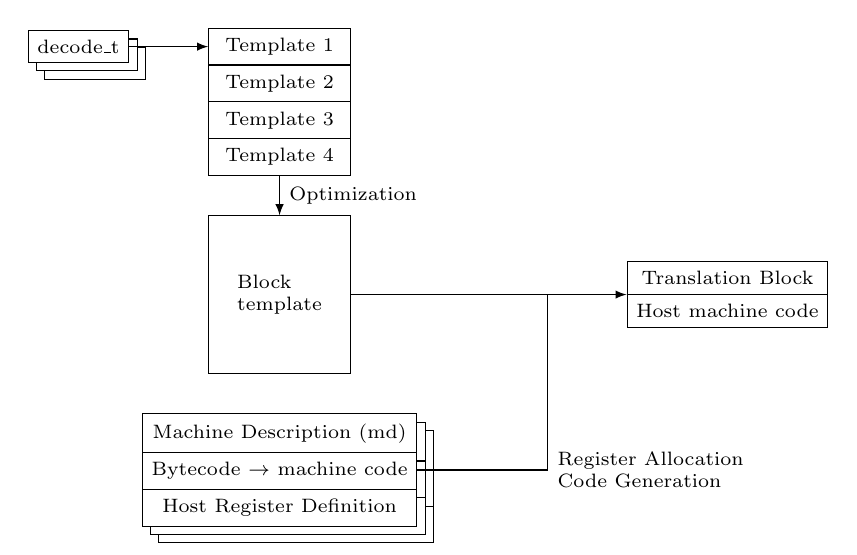
\begin{tikzpicture}[font=\scriptsize, >=latex, node distance=1.cm]

\node[draw, double copy shadow={shadow xshift=3pt,shadow yshift=-3pt}, fill=white] (decode) {decode_t};
\node[rectangle split, rectangle split parts=4, draw, right=of decode, anchor=text west, minimum width=1.8cm] (templates) {Template 1\nodepart{two} Template 2\nodepart{three} Template 3\nodepart{four} Template 4};
\draw[->] (decode) -- (templates.text west);

\node[draw, below=0.5cm of templates, minimum height=2cm, align=left, minimum width=1.8cm] (opt-template) {Block\\template};
\draw[->] (templates) -- (opt-template) node[midway, right] {Optimization};

\node[rectangle split, rectangle split parts=3, align=left, draw, below=0.5cm of opt-template, double copy shadow={shadow xshift=3pt,shadow yshift=-3pt}, fill=white] (md) {Machine Description (md)\nodepart{two} Bytecode $\rightarrow$ machine code\nodepart{three} Host Register Definition};

\coordinate[right=2.5cm of opt-template] (junction);

\node[draw, right=1cm of junction, rectangle split, rectangle split parts=2,] (host-code) {Translation Block\nodepart{two} Host machine code};

\draw[->] (md) -| node[pos=0.5, right, align=left] {Register Allocation\\Code Generation} (junction) -- (host-code);
\draw[] (opt-template) -- (junction);

\end{tikzpicture}
\end{frame}

\begin{frame}{Optimizations}
\centering
\inputpicture{bt-optimization}
\end{frame}

\begin{frame}{Connection between Translation Blocks}
\centering
\inputpicture{bb-translation}
\end{frame}

\begin{frame}{Why Optimizations During BT Are Complicated?}

\begin{itemize}
\item Machine code has less information about the algorithm compared to code in
  high-level programming languages.
\item Many compiler optimizations cannot be used.
% TODO: Examples with clarification.
\item BT optimizations are limited in time.
\end{itemize}
\pause
\begin{itemize}
\item Variable addresses --- not available.
\item Function boundaries --- not available.
\item Branch addresses --- partially known.
\end{itemize}
\end{frame}

\section*{Conclusions}

\begin{frame}{Conclusions}
\begin{itemize}
\item Basic 5-stage pipeline.
\item Decoder, disassembler, encoder.
\item Switched interpreter.
\item Threaded interpreter.
\item Cached interpreter.
\item Exeption, Interrupt, Trap, Fault\dots
\item Interpretation, Compilation, Translation.
\item Binary Translation.
\item Static and Dynamic Binary Translation.
\item Template, Capsule.
\item Intermediate Representation.
\end{itemize}
\end{frame}

\begin{frame}[allowframebreaks]{Bibliography}
\begin{thebibliography}{99}
  \bibitem{} \textit{D. Mihoka, S. Shwartsman}. Virtualization Without Direct
    Execution or Jitting: Designing a Portable Virtual Machine Infrastructure.
  \bibitem{} \textit{Y. Lifshitz, R. Cohn, I. Livni, O. Tabach, M. Charney, K.
    Hazelwood}. Zsim: A Fast Architectural Simulator for ISA Design-Space
    Exploration.
  \bibitem{} \textit{F. Larsson, P. Magnusson, B. Werner}. SimGen: Development of
    Efficient Instruction Set Simulators.
  \bibitem{} \textit{A. Sepp, J. Kranz, A. Simon}. GDSL: A Generic Decoder
    Specification Language for Interpreting Machine Language.
  \bibitem{} \textit{Jim Smith and Ravi Nair}. Virtual Machines: Versatile
  Platforms for Systems and Processes.
  \bibitem{} \textit{Fabrice Bellard}. QEMU, a Fast and Portable Dynamic
  Translator.
  \bibitem{} \textit{Anton Chernoff and Ray Hookway.} {DIGITAL FX!32} Running
  32-Bit x86 Applications on {Alpha} {NT}.
  \bibitem{} \textit{Leonid Baraz [et al.]} IA-32 Execution Layer: a Two-Phase
  Dynamic Translator Designed to Support IA-32 Applications on
  Itanium\reg-Based Systems.
\end{thebibliography}
\end{frame}

\finalslide

\end{document}
